\chapter{The Pacific Ocean Neutrino Explorer}

The  Pacific Ocean Neutrino Explorer (P-ONE) is a proposed Neutrino Telescope planned to run in the Pacific Ocean near the West Coast of Vancouver Island, Canada \cite{pone}. As with other Neutrino Telescopes, P-ONE hopes to detect and characterize astrophysical neutrinos from galactic and extra-galactic sources for extremely high energy neutrinos \cite{pone}. In particular, due to the planned multi-cubic kilometer coverage, it would be suitable for neutrinos from sources such as Blazars \cite{icecube_nat}. Moreover P-ONE hopes to provide an avenue for research in exotic particle searches, dark matter, neutrino oscillations, supernova neutrinos, tau neutrino studies ($\nu_{\tau}$) and oceanography studies \cite{pone}. 

\section{Geometry}

The geometry of the detector is incredibly important, as the layout and positions of the detectors can drastically change the results and the sensitivies \cite{icecube}. The first proposed Explorer phase for P-ONE corresponds to the first 10 string-segment to be deployed \cite{pone}. Each string will be composed of 20 photo-sensors and atleast two calibration modules \cite{pone}, with the strings organized in an array similar to that of IceCube \cite{pone,icecube}. In order to avoid using thousands of strings to get a larger coverage, it can achieve a similar amount of information using a segmented approach where 6 more arrays similar to those of the Explorer are added around it \cite{pone}. This design is drawn in Figure \ref{fig:pone_geo}. 

\begin{figure}[h]
  \centering
  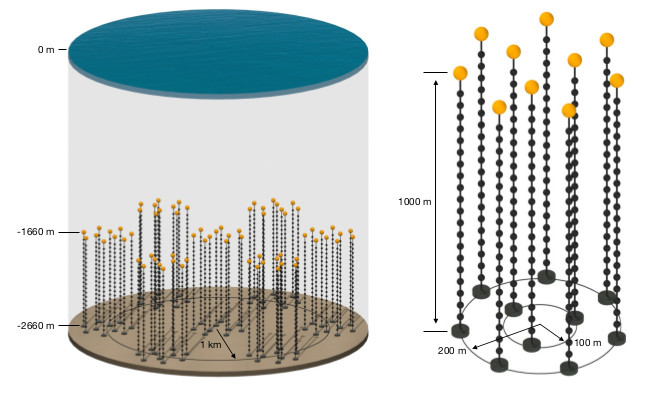
\includegraphics[width=12cm]{./Figures/PONEv0_-23_design.jpg}
  \caption{Left: Proposed full detector of the P-ONE detector. Right: Proposed array for the Explorer deployment of P-ONE.}
  \label{fig:pone_geo}
\end{figure}

With the current proposed geometry, the detector will be incredibly sensitive to horizontal incoming high energy muons from neutrino astrophysical neutrino sources \cite{pone}. 

\section{Detectors}
Similar to previously constructed Neutrino Telescopes, P-ONE will primarily use Vavilov-Cherenkov Radiation from leptons produced through neutrino interactions. This electromagnetic radiation is then detected through highly sensitive optical modules that consist of Photo-Multiplier Tubes (PMTs).

\subsection{Photo-Multiplier Tubes}



\subsection{Digital Optical Modules}

Adopted from the DOMs in IceCube that house the PMTs.

\subsection{mDOMs}

Proposed redesign of the IceCube DOM to increase the granularity of light detection. In place of one large PMT, multiple smaller PMTs can line the same space and coverage at the cost of gaps between detectors. The benefit being that individual hits on the smaller PMTs can provide extra information using the acceptance angle and directionality of that particular PMT. Moreover, in theory this can also reproduce the standard DOM data as the signal collected by a single PMT in the array can be collected and treated as a hit for the entire DOM. This gives the mDOMs a felxibility that isn't present for standard DOMs. In IceCube the standard DOMs use single $10^{\prime\prime}$ diameter PMTs \cite{icecube}, where the mDOMs would use multiple $3^{\prime\prime}$ diameter PMTs. 

\section{Strings for Absorption length in Water}

The Pathfinder mission for P-ONE is the STRings for Absroption length in Water (STRAW) and its follow up STRAW-b, which were deployed in 2018 and 2020 respectively. The purpose of these missions was to test the technical details of running an experiment like P-ONE, such as the hardware limitation, to provide data to measure the Attenuation length of light in water for light in wavelengths between 350 nm and 600 nm, characterize the bioluminescence of deap-sea living organisms and the $^{40}$K dissolved in the salty water \cite{straw}.

The basic design of STRAW is the same as that of standard Neutrino Telescopes; using PMTs for detecting photons and calibrating light emmitting sources on mooring lines to collect data \cite{straw}. In this particular case STRAW uses two vertical mooring lines with $3^{\prime\prime}$ PMTs and Precision Optical Calibrationn Modules (POCAMs) for the calibration sources \cite{straw}, which provide isotropic and short pulsed flashes of light. The attenuation length $L_{T}$ in water can be realized using the known photon intensity $N_{0}$, the wavelength from the POCAM flashes and the distance $r$ to each particular PMT with effective collection area $A_{\text{det}}$ measuring an intensity $N(r)$ \cite{straw}. This yields
\begin{equation}
  N(r) = \frac{N_{0}}{4\pi r^{2}}\exp\left(-\frac{r}{L_{T}}\right)A_{\text{det}}\, .
\end{equation}



\section{Ocean Networks Canada}

Ocean Networks Canada (ONC) is the institution that has supported and provided infrastructure for running an experiment of the scale that P-ONE is. 


